\documentclass{report}
\usepackage{epsfig,graphics,fancybox,amsmath,hyperref,ulem,tabularx,color,graphicx,multirow,colortbl,soul}
\newcommand{\hili}[1]{\colorbox{yellow}{#1}}


\normalem
%\input /home/jaosborn/research/mymacs.tex
\input mymacs.tex
\def\defn{\noindent\underline{Definition}: }
\def\gmeanb{\bar{y}_{+++}}
\def\tmean#1{\bar{y}_{#1+}}
\def\Tmean#1{\bar{Y}_{#1+}} 
\def\h0sim{\stackrel{H_0}{\sim}}
\def\abg#1{(\alpha\beta\gamma)_{#1}}

\makeatletter
\def\hlinewd#1{%
\noalign{\ifnum0=`}\fi\hrule \@height #1 %
\futurelet\reserved@a\@xhline} 
\makeatother

\setlength{\textwidth}{6.5in}
\setlength{\textheight}{8.5in}
\setlength{\parindent}{0pt}

\begin{document}
\setlength{\topmargin}{0pt}
\setlength{\oddsidemargin}{0pt}

\newpage
\pagenumbering{arabic}

\begin{center}\Huge\textbf{Problems with worked out solutions for Regression and Correlation.}\\
\normalsize \end{center}
\large ~\hrulefill
~\\
\textbf{An example: The association between corn yield and rainfall:}\\~\\
Yields $y$ (in bushels/acre) on corn raised in six midwestern states from 1890 to 1927 recorded with rainfall $x$ (inches/yr). \\
$$ y_1,\ldots,y_{38} \ \ \ \mbox{and} \ \ \  x_1,\ldots,x_{38}.$$
\begin{center}
\begin{tabular}{|c|cccccccccc|} \hline
Year & 1890 & 1891 & 1892 & 1893 & 1894 & 1895 & 1896 & 1897 & 1898 & 1899 \\
Yield  & 24.5 & 33.7 & 27.9 & 27.5 & 21.7 & 31.9 & 36.8 & 29.9 & 30.2 & 32\\
Rainfall & 9.6 & 12.9 & 9.9 & 8.7 & 6.8 & 12.5 & 13 & 10.1 & 10.1 & 10.1  \\  \hline
Year & 1900 & 1901 & 1902 & 1903 & 1904 & 1905 & 1906 & 1907 & 1908 & 1909 \\
Yield  & 34 & 19.4 & 36 & 30.2 & 32.4 & 36.4 & 36.9 & 31.5 & 30.5 & 32.3\\
Rainfall & 10.8 & 7.8 & 16.2 & 14.1 & 10.6 & 10 & 11.5 & 13.6 & 12.1 & 12 \\ \hline
Year & 1910 & 1911 & 1912 & 1913 & 1914 & 1915 & 1916 & 1917 & 1918 & 1919 \\
Yield & 34.9 & 30.1 & 36.9 & 26.8 & 30.5 & 33.3 & 29.7 & 35 & 29.9 & 35.2\\
Rainfall & 9.3 & 7.7 & 11 & 6.9 & 9.5 & 16.5 & 9.3 & 9.4 & 8.7 & 9.5 \\ \hline
Year & 1920 & 1921 & 1922 & 1923 & 1924 & 1925 & 1926 & 1927 & &\\
Yield & 38.3 & 35.2 & 35.5 & 36.7 & 26.8 & 38 & 31.7 & 32.6 & &\\
Rainfall & 11.6 & 12.1 & 8 & 10.7 & 13.9 & 11.3 & 11.6 & 10.4 & &\\ \hline
\end{tabular}
\end{center}

A {\em scatter plot} provides a visual for inspecting the association between $Y$ and $X$.  
\begin{center}
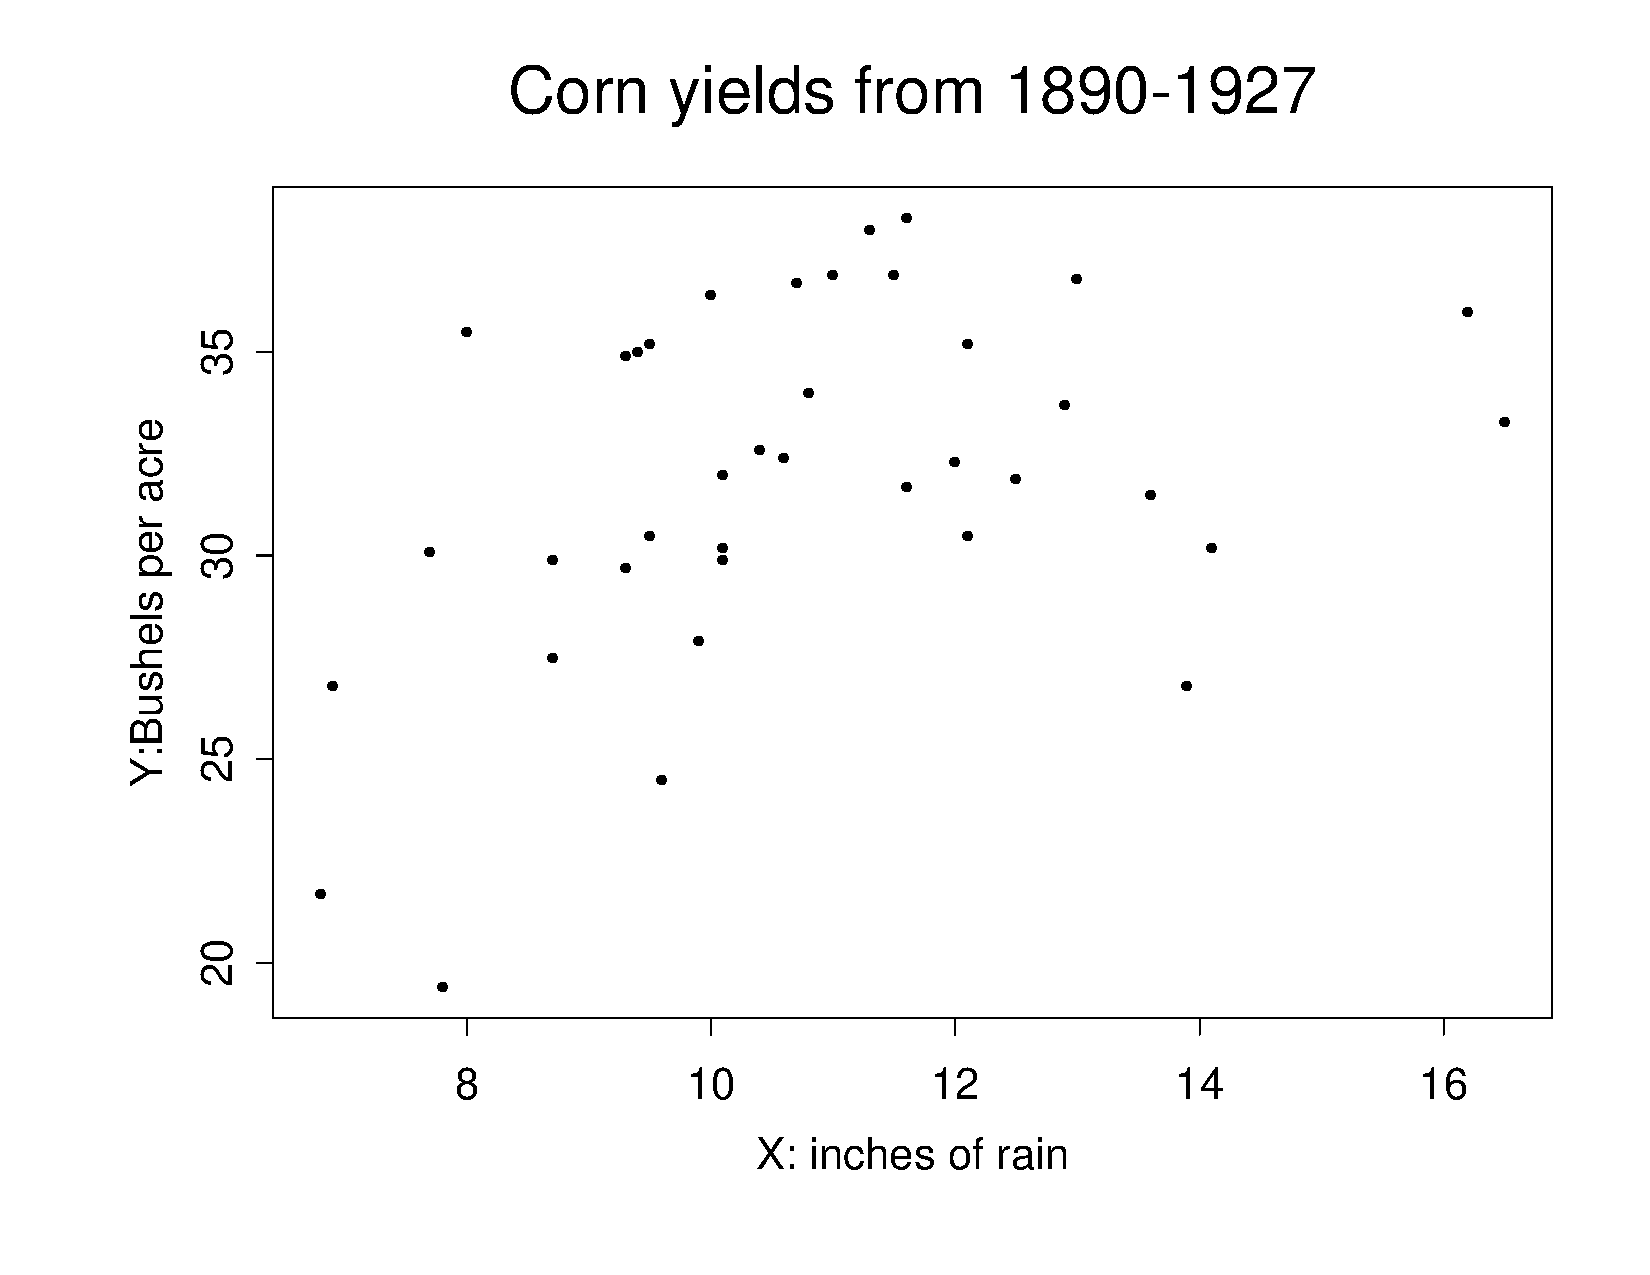
\includegraphics[scale=0.3]{cornyield.pdf}
\end{center}
From the scatter plot, the form of the association appears to be linear or slightly quadratic, the strength is weak to moderate, and the direction is positive.\\~\\

A correlation analysis was done and a SLR model was fit using SAS yielding the following (partial) output:
\begin{small}
\begin{verbatim}
proc corr data=corn cov;          proc reg data=corn;
var yield rain;                   model yield=rain;
run;                              run;
\end{verbatim}
\end{small}

\begin{center}
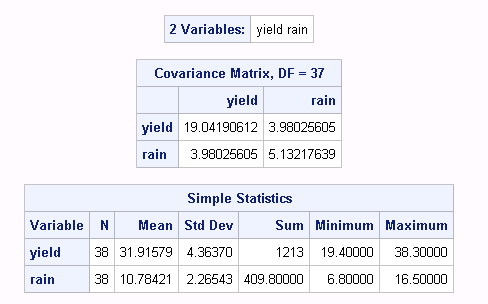
\includegraphics[scale=0.7]{cornsummary}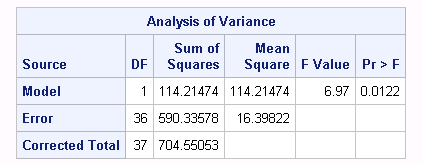
\includegraphics[scale=0.7]{cornslranova}
\end{center}


Use the output to 
\begin{enumerate}
\item Find the value of the correlation coefficient.  
\item Find the 95\% confidence interval for the population correlation, $\rho$.  Interpret the interval you found.
\item Without conducting a hypothesis test, use the confidence interval to make a conclusion about the hypotheses $H_0: \rho=0$ vs $H_A: \rho\neq 0$.
\item Find the fitted line for the SLR with yield as the response and rainfall as the predictor.
\item Use the summary statistics to create 95\% confidence intervals for $\beta_1$ and $\beta_0$.  Note: $t_{36, 0.025}=2.028$.
\item Find a 95\% confidence interval for the true mean yield for corn from the six states for a rainfall of 14inches.
\item Suppose the rainfall collected for a year was 14 inches but the yield of the corn from the six states was not recorded.  Find a 95\% prediction interval for the yield of the corn from that year.
\end{enumerate}

\newpage

Solutions:
\begin{enumerate}
\item From the output we have
$$ \bar{x}=10.78, \ \ \ s^2_X=5.13 \ \ s_X = 2.27$$
$$ \bar{y}=31.92, \ \ \ s^2_Y=19.04 \ \ s_Y = 4.36$$ 
$$ s_{XY}=3.98$$
Applying the formula for $r$, we get
$$ r=\frac{s_{XY}}{s_X s_Y}=\frac{3.98}{\sqrt{5.13 \times 19.04}} =0.40$$

\item With $r=0.40$, $n=38$, and $z_{\alpha/2}=1.96$, a $95\%$ interval is given by
$$ \left(\frac{\frac{1+0.4}{1-0.4}e^{-2*1.96/\sqrt{38-3}}-1}{\frac{1+0.4}{1-0.4}e^{-2*1.96/\sqrt{38-3}}+1}, \frac{\frac{1+0.4}{1-0.4}e^{2*1.96/\sqrt{38-3}}-1}{\frac{1+0.4}{1-0.4}e^{2*1.96/\sqrt{38-3}}+1}\right)=(0.09,0.64).$$
We are 95\% confident that the true correlation between corn yield and rainfall is between 0.09 and 0.64.
\item Since there is a one-to-one correspondence between a two-sided HT at the 0.05 level and a $100(1-\alpha)$\% CI, we would reject $H_0:\rho=0$ as 0 is not in the interval.\\~\\

\item To find the fitted least squares line:
\begin{eqnarray*}\hat{\beta}_1 &=& \frac{s_{xy}}{s_x^2} \\
&=& \frac{3.98}{5.13} =0.776 (\mbox{ bushels per acre }\div \mbox{ inches per year})\\
or &=& r_{xy}\frac{s_y}{s_x} \\
&=& (0.40) \sqrt{\frac{19.04}{5.13}}\\
&=& 0.771 \mbox{(off due to rounding)}\\
\hat{\beta}_0 &=& \bar{y}-\hat\beta_1 \bar{x}\\
&=& 31.92- 0.776 (10.78) \\
&=& 23.555 \mbox{ bushels per acre } 
\end{eqnarray*}
yielding the least squares line of
$$ \hat{y}=23.555 + (0.776) x. $$

\item To find confidence intervals for the regression parameters:\\
For $\beta_1$, note that \\
$$S_{xx}=(n-1)s_x^2=5.13(38-1)=189.81$$
and we can estimate $\sigma^2$ using the $MS(E)=16.40$.  Thus, a 95\% CI for $\beta_1$ is given by
$$0.776 \pm 2.028 \sqrt{\frac{16.40}{189.81}} =(0.180, 1.372)$$
We are 95\% confident the true value of the slope lies in this interval.
For $\hat{\beta}_0$,
$$ 23.555 \pm 2.028 \sqrt{16.40\left(\frac{1}{38}+\frac{(10.78)^2}{189.81}\right)} =(16.992, 30.118)$$
\item First we can find the point estimate 
$$\hat\mu(14)=23.555+0.776*14 =  34.419$$ 
The standard error of this mean estimate is 
$$ \sqrt{16.40\left(\frac{1}{38}+\frac{(14-10.78)^2}{189.81}\right)}=1.125  $$
Thus, a 95\% CI for the mean corn yield for 14 inches of rain is
$$34.419 \pm 2.028*1.125 = (32.138, 36.701)$$
We are 95\% confident that the true mean corn yield for all years with 14 inches of rain is between 32.138 and 36.701 bushels per acre.
\item A $95\%$ prediction interval is then
$$ 34.419 \pm 2.028 \sqrt{16.40\left(1+\frac{1}{38}+\frac{(14-10.78)^2}{189.81}\right)}=(25.880, 42.958) $$
We are 95\% confident that a year that has 14 inches of rain will have a yield between 25.880 and 42.958 bushels per acre.
\end{enumerate}

\newpage

Looking at the scatter plot, there may be a quadratic relationship.  We can fit a linear regression model with rainfall and rainfall squared as predictors to investigate this. Use the following SAS output to conduct a LOF test for the SLR model.
\begin{small}
\begin{verbatim}
data corn;               proc reg data=corn;
set corn;                model yield= rain rain2/ss1;
rain2=rain*rain;         run;
run;
\end{verbatim}
\end{small}

\begin{center}
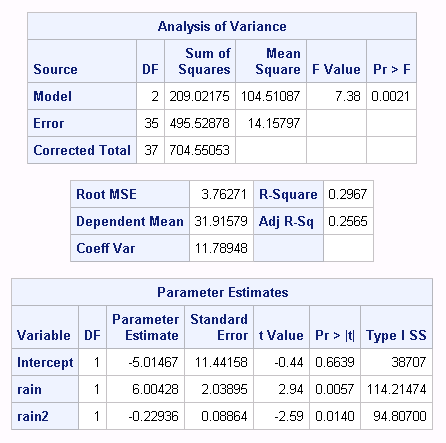
\includegraphics[scale=0.7]{cornquadratic}
\end{center}

The $F$ statistic for the LOF test can be written as
$$F=\frac{\frac{SS(R)_f-SS(R)_r}{p-q}}{MS(E)_f}=\frac{\frac{209.02-114.21}{2-1}}{14.16}=6.70$$
We compare this to the critical value from the appropriate $F$ distribution: $F_{1,35,0.05}=4.12$\\~\\
Therefore, we reject $H_0:\beta_2=0$ in favor of $H_A:\beta_2\ne0$.\\~\\
Note: This test statistic of 6.70 is equivalent to the t-test squared $(-2.59)^2$ since we only have 1 numerator degree of freedom.

\newpage

A couple random questions:
\begin{enumerate}
\item What type of data is needed to run a MLR model?
\item An industrial quality control expert takes 200 hourly measurements on an industrial furnace which is under control and finds that a $95\%$ confidence interval for the mean temperature is (500.35, 531.36). As a result he tells management that the process should be declared out of control whenever hourly measurements fall outside this interval and, of course, is later fired for incompetence. (Why and what should he have done?)
\end{enumerate}

Solutions:
\begin{enumerate}
\item The data situation needed for a MLR model is $p$ quantitative predictors and 1 quantitative response measured on the same individuals (i.e. units).
\item The interval found is for the \textbf{mean} temperature.  The interval is not trying to capture a single new observation.  The interval that should have been found is a prediction interval.  This interval will be much wider as it is much more difficult to predict a new value as opposed to predicting the true mean.
\end{enumerate}

\newpage

\textbf{The classical regression example - The association between height of adults and their parents}
\begin{center}
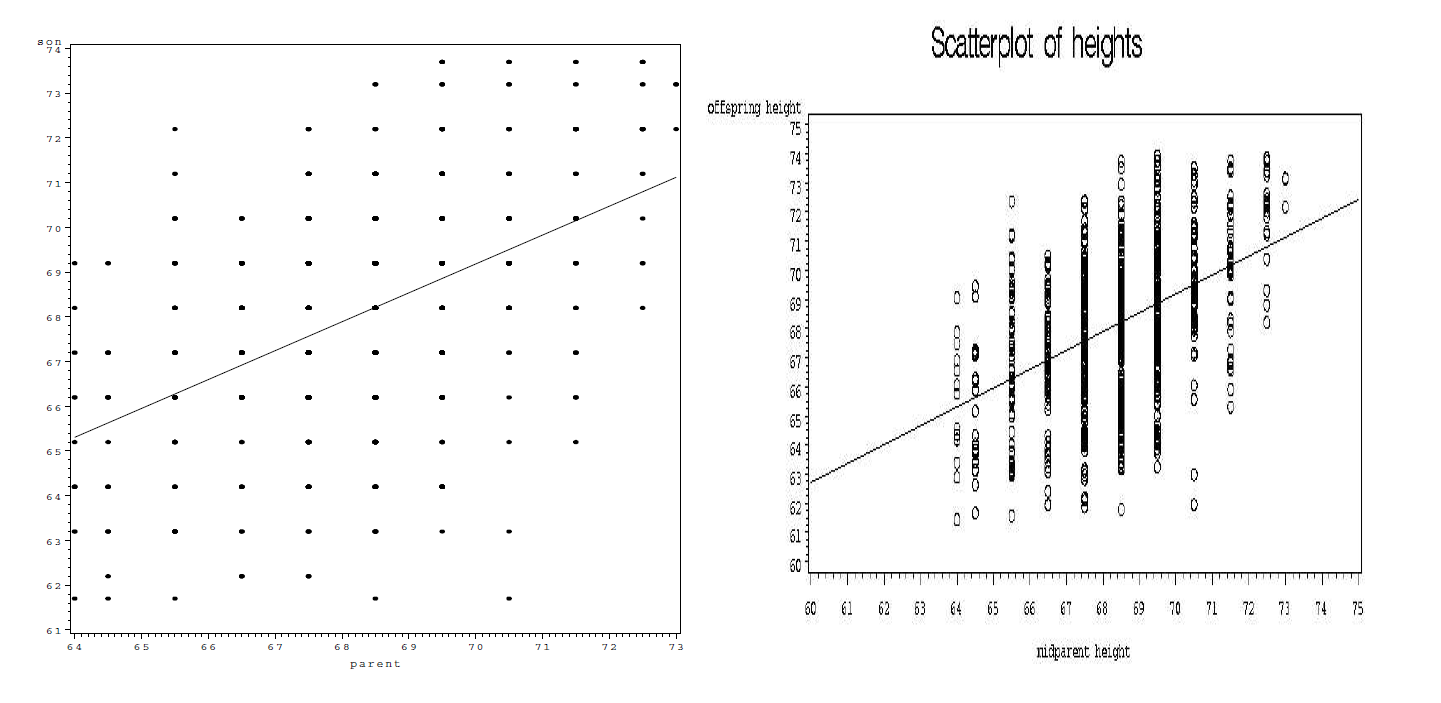
\includegraphics[scale=0.4]{galton}
\begin{small}
\begin{verbatim}

/* -------------------------------------------------------------------
|  Stigler , History of Statistics pg. 285 gives Galton's famous data |
| on heights of sons (columns,Y) and average parents' height (rows,X) |
| scaled to represent a male height (essentially sons' heights versus |
| fathers' heights).   Taken from Dickey's website.                   |
\ -------------------------------------------------------------------*/

    61.7 62.2 63.2 64.2 65.2 66.2 67.2 68.2 69.2 70.2 71.2 72.2 73.2 73.7
73.0  0    0    0    0    0    0    0    0    0    0    0    1    3    0
72.5  0    0    0    0    0    0    0    1    2    1    2    7    2    4
71.5  0    0    0    0    1    3    4    3    5   10    4    9    2    2
70.5  1    0    1    0    1    1    3   12   18   14    7    4    3    3
69.5  0    0    1   16    4   17   27   20   33   25   20   11    4    5
68.5  1    0    7   11   16   25   31   34   48   21   18    4    3    0
67.5  0    3    5   14   15   36   38   28   38   19   11    4    0    0
66.5  0    3    3    5    2   17   17   14   13    4    0    0    0    0
65.5  1    0    9    5    7   11   11    7    7    5    2    1    0    0
64.5  1    1    4    4    1    5    5    0    2    0    0    0    0    0
64.0  1    0    2    4    1    2    2    1    1    0    0    0    0    0
\end{verbatim}
\end{small}
\end{center}

Many questions we could answer using this dataset: Note: $t_{927,0.025}\approx t_{926,0.025}=1.963$
\begin{enumerate}
\item Suppose we ignore midparent height $x$.  Consider estimating the mean $\mu_{Y}=E(Y)$.  Use ST 511 knowledge to obtain a confidence interval for the mean height of the sons.  (Use summary statistics in the output that follows to complete this naive analysis.)\\

\newpage

\noindent For the rest of the problems, consider a linear regression between the sons' heights and the midparent height.  Let $Y_1,\ldots,Y_n$ denote the sons' heights.  Given their average parent height, $X=x_i$,
$$ Y_i = \beta_0 + \beta_1 x_i + E_i \ \ \ \mbox{ for }i=1,\ldots,n (n=928).$$
where $E_1,\ldots,E_n$ are $iid$ Normal with mean 0 and variance $\sigma^2$.\\~\\
Output is given on the following pages, use it to answer the following:\\
\item What is the meaning, in words, of $\beta_1$?
\item True/false: (a) $\beta_1$ is a statistic (b) $\beta_1$ is a parameter (c) $\beta_1$ is unknown.
\item What is the observed value of $\hat\beta_1$?
\item True/false: (a) $\hat\beta_1$ is a statistic (b) $\hat\beta_1$ is a parameter (c) $\hat\beta_1$ is unknown.
\item Is $\hat\beta_1=\beta_1$?
\item How much does $\hat\beta_1$ vary about $\beta_1$ from sample to sample?  (Provide an estimate of the standard error, as well as an expression indicating how it was computed.)
\item What is a region of plausible values for $\beta_1$ suggested by the data? (i.e. a CI)
\item What is the line that best fits these data, using the criterion that smallest sum of squared residuals is ``best?''
\item How much of the observed variation in the heights of sons (the $y$-axis) is explained by this ``best" line?
\item Give an expression in terms of the parameters of the model for the true average height of sons with midparent height $x=68$.
\item What is the estimated average height of sons whose midparent height is $x=68$?
\item Is this the true average height in the whole population of sons whose midparent height is $x=68$?
\item What is the estimated standard deviation among the population of sons whose parents have midparent height $x=68$?  
\item What is the estimated standard deviation among the population of sons whose parents have midparent height $x=72$?  
Bigger, smaller, or the same as that for $x=68$?
\item What is the estimated standard error of the estimated average height for sons with midparent height $x=68$, i.e. $\hat\mu(68)=\hat\beta_0 + 68 \hat\beta_1$?
Provide an expression for this standard error.
\item Is the estimated standard error of $\hat\mu(72)$ bigger, smaller, or the same as that for $\hat\mu(68)$?
\item What quantity can you use to describe or characterize the linear association between height and midparent height in the whole population?
Is this a parameter or a statistic?
\item Is the observed linear association between son's height and midparent height strong?  To answer, report the value of r and the p-value from the appropriate test.
\item Define $\mu_Y,\sigma_Y,\mu_X,\sigma_X,\rho$. Parameters or statistics?
\item What are plausible values for $\rho$ suggested by the data? (i.e. form a CI)
\item Is \fbox{$E_1,\ldots,E_{928} \iid N(0,\sigma^2)$} a reasonable assumption?
\item Based \textbf{solely} on this study, can we conclude that larger parents cause larger sons?
\end{enumerate}

\begin{center}
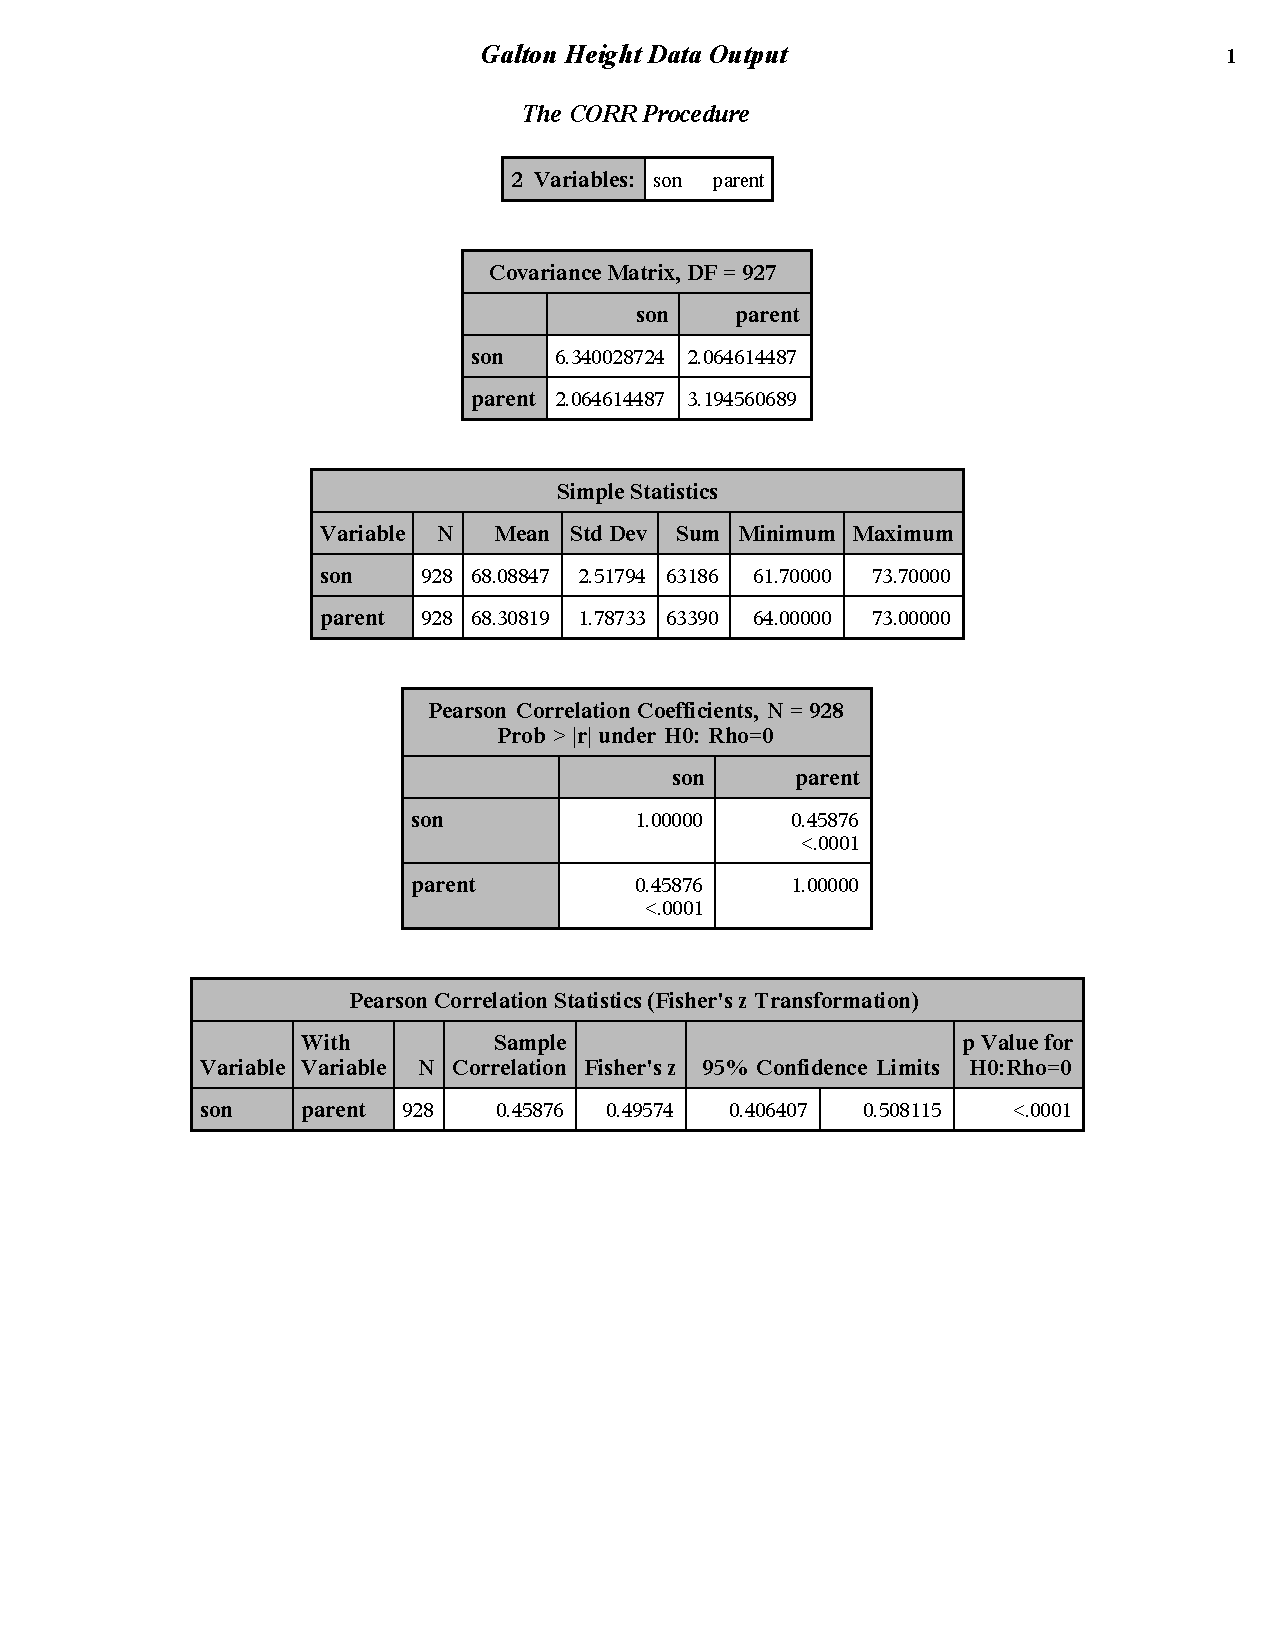
\includegraphics[page=1,scale=0.8,trim= 10mm 50mm 10mm 10mm]{GaltonSAS}\\
\includegraphics[page=2,scale=0.8,trim= 10mm 10mm 10mm 10mm]{GaltonSAS}\\
\includegraphics[page=3,scale=0.8,trim= 10mm 10mm 10mm 10mm]{GaltonSAS}\\
\includegraphics[page=4,scale=0.5,trim= 10mm 100mm 10mm 20mm]{GaltonSAS}\\
\includegraphics[page=5,scale=0.5,trim= 10mm 100mm 10mm 20mm]{GaltonSAS}\\
\includegraphics[page=6,scale=0.7,trim= 10mm 240mm 10mm 5mm]{GaltonSAS}
\end{center}

\newpage

\textbf{Answers to questions from simple linear regression:}
\begin{enumerate}
\item A CI for a mean when the true standard deviation is unknown is 
$$\bar{y}\pm t_{n-1,\alpha/2}s/\sqrt{n}= 68.09 \pm 1.963*2.52/\sqrt{928}=(67.928,68.252)$$
\item Change in average son's height (inches) per one inch increase in 
midparent height.
\item $\beta_1$ is an unknown parameter. 
\item $\hat\beta_1=0.65$ son inches/midparent inch.
\item $\hat\beta_1=0.65$ is an observed value of a statistic. 
\item 
$\beta_1$ is the slope of the population mean, 
$\hat\beta_1$ is the slope from the SLR of the observed data.
$\hat\beta_1=\beta_1$ is very unlikely.
\item $\widehat{SE}(\hat\beta_1) = \sqrt{MS[E]/S_{xx}}=0.041$.
\item Add and subtract 1.963 times the SE to get $(0.566,0.727)$
\item $\hat{y}=23.942 + 0.646 x$
\item $r^2=0.2105$
\item $\mu(68)=\beta_0+ 68 \beta_1$
\item $\hat{\mu}(68)=\hat\beta_0+68 \hat\beta_1=67.889$
\item Probably not! $\mu(68)=\beta_0+ 68 \beta_1$ is unknown and $\hat{\mu}(68)$ is only an estimate.
\item This question is asking for the square root of the estimate of variation due to experimental error or $\hat{\sigma}=\sqrt{MS[E]}=2.24$.
\item Same as the previous question as an assumption on our model is that the errors have the same variance (and hence square root) at every point on the line.  (Assumption of homoskedasticity.)
\item $\hat{SE}(\hat\beta_0+ 68 \hat\beta_1)=0.075$.
Expressions given by
\begin{eqnarray*}
\widehat{SE}(\hat\mu(68)) &=& \sqrt{MS[E]\left(\frac{1}{n}+\frac{(68-\bar{x})^2}{\sum(x_i-\bar{x})^2}\right)}\\
&=& \sqrt{(1,68)' MS[E] (X'X)^{-1} (1,68)}
\end{eqnarray*}
$X$ a $(928 \times 2)$ {\em design matrix}.
\item $\widehat{SE}(\hat\mu(72)) > \widehat{SE}(\hat\mu(68))$ as it is further from $\bar{x}$, where we have the most information about our data.
\item $\rho$, which is the population correlation coefficient (a parameter).
\item $r=0.459$, moderate, positive.  P-value $<$ 0.0001, there is a significant linear relationship.
\item These are all parameters and describe the mean and standard deviation of the sons` heights, the mean and standard deviation of the midparent`s heights, and the correlation between them.
\item The confidence interval is 
$$ \left(\frac{\frac{1+r}{1-r}e^{-2z/\sqrt{n-3}}-1}{\frac{1+r}{1-r}e^{-2z/\sqrt{n-3}}+1}, 
\frac{\frac{1+r}{1-r}e^{2z/\sqrt{n-3}}-1}{\frac{1+r}{1-r}e^{2z/\sqrt{n-3}}+1}\right)$$
or $(0.406,0.508)$.
\item Residuals reasonably symmetric, no heavy tails.  Model fit is ok.
\item Based on this study alone, no.  This is an observational study as no midparent heights were assigned by the researchers.  However, if science and genetics are brought in, a causal relationship might be inferred.
\end{enumerate}

\newpage

Recall the example about a random sample of students taking the same exam:
\begin{center}
\begin{tabular}{|c|c|c|} \hline
IQ & TIME & GRADE \\ \hline
105 & 10 & 75 \\
110 & 12 & 79 \\
120 & 6 & 68 \\
116 & 13 & 85 \\
122 & 16 & 91 \\
130 & 8 & 79 \\
114 & 20 & 98 \\
102 & 15 & 76 \\ \hline
\end{tabular}
\end{center}
\noindent
Consider the additive regression model for the GRADE of 
subject $i$, $Y_i$, in which the mean of $Y_i$ is a linear function of IQ and Time ($X_{i1}=\mbox{IQ}$ and $X_{i2}=\mbox{TIME}$) for subjects $i=1,\ldots,8$:
$$ Y = \beta_0 + \beta_1 \mbox{IQ} + \beta_2 \mbox{TIME} + \mbox{error}$$ 
or
$$ Y_i = \beta_0 + \beta_1 X_{i1} + \beta_2 X_{i2} + E_{i} $$ 
Let`s write out the model in matrix form:
\begin{center}
\begin{tabular}{ccc}
\textbf{y}=$\left(\begin{array}{c} 75 \\79\\68\\85\\91\\79\\98\\76\\\end{array}\right)$ &
\textbf{X}=$\left(\begin{array}{ccc}
1  &  105  &   10  \\
1  &  110  &   12  \\
1  &  120  &    6  \\
1  &  116  &   13  \\
1  &  122  &   16  \\
1  &  130  &    8  \\
1  &  114  &   20  \\
1  &  102  &   15  \\
\end{array}\right)$&
$\boldsymbol{\beta}$=$\left(\begin{array}{c} \beta_0 \\\beta_1\\\beta_2\\\end{array}\right)$ 
\end{tabular}
\end{center}

$$\textbf{X}'\textbf{X}=\left(\begin{array}{rrr} 
8      &        919      &        100\\
919    &       106165    &        11400 \\
100    &        11400    &         1394  \\
\end{array}\right)$$ 
$$(\textbf{X}'\textbf{X})^{-1}=\left(\begin{array}{rrr} 
28.90  &   -0.23  &   -0.22  \\
-0.23  &   0.0018  &   0.0011  \\
-0.22  &   0.0011  &   0.0076  \\
\end{array}\right)$$
$$ (\textbf{X}'\textbf{X})^{-1} \textbf{X}'\textbf{Y} = \left(\begin{array}{r} 0.74 \\ 0.47 \\ 2.10
\end{array}\right)$$
$$ SS(E) = \textbf{e}'\textbf{e} = (\textbf{Y}-\hat{\textbf{Y}})'(\textbf{Y}-\hat{\textbf{Y}}) = 45.8, \ \  \textbf{e}'\textbf{e}/df = 9.15$$
\bigkn
$$ \widehat{\boldsymbol{\Sigma}} = MS(E) (\textbf{X}'\textbf{X})^{-1} = \left(\begin{array}{rrr} 
264.45  &   -2.07   &  -2.05 \\
-2.07  &    0.017   &   0.010 \\
-2.05  &    0.010   &  0.070 \\
\end{array}\right)$$

\newpage

Some questions to answer:
\begin{enumerate}
\item What is the estimate for $\beta_1$?  Interpretation? 
\item What is the standard error of $\hat\beta_1$?  
\item Is $\beta_1=0$ plausible, while controlling for possible linear associations between Test Score and Study time? ($t_{0.025,5}=2.57$) 
\item Estimate the mean grade among the population of ALL students with $IQ=113$ who study $TIME=14$ hours.
\item Report a standard error for this mean.
\item Report a $95\%$ confidence interval for this mean.
\item What is the estimate of the error variance?
\end{enumerate}
~\\
Some answers:
\begin{enumerate}
\item $\hat\beta_1 =0.47$ (second element of $(\textbf{X}'\textbf{X})^{-1} \textbf{X}'\textbf{Y}$, estimated average exam points per IQ point increase for students studying the same amount)
\item $\sqrt{0.017}=0.13$ (square root of middle element of $\widehat{\boldsymbol{\Sigma}}$)
\item $H_0: \beta_1=0~~~vs ~~~H_A:\beta_1\neq 0$, T-statistic: $t=(\hat\beta_1 - 0)/\hat{SE}(\hat\beta_1)$ \\
Observed value is $t=.47/\sqrt{.017} = .47/.13=3.6 > 2.57$ (``$\hat\beta_1$ differs significantly from 0.'')
\item Unknown population mean: $\mu(113,14)=\beta_0+\beta_1(113) +\beta_1(14)$ \\
Estimate : $\hat\mu(113,14)=(1,113,14)* \hat\beta = 83.6$
\item $\hat{Var}((1,113,14) * \hat{\boldsymbol{\beta}}) = (1,113,14)\widehat{\Var}(\hat{\boldsymbol{\beta}}) (1,113,14)'$\\
or $(1,113,14)\widehat{\boldsymbol{\Sigma}} (1,113,14)'=1.3$ or $SE(\hat\theta) = \sqrt{1.3}=1.14$
\item $\hat\mu(113,14) \pm t(0.025,5) \hat{SE}(\hat\mu(113,14)) \ \mbox{ or } \ 83.6 \pm { 2.57} (1.14) \ \mbox{ or } \ (80.7, 86.6)$
\item The estimate of the error variance is the $MS(E)=9.15$
\end{enumerate}

\newpage

Continuing this example, consider this sequence of analyses: 
\begin{enumerate}
\item Regress GRADE on IQ. 
\item Regress GRADE on IQ and TIME. 
\item Regress GRADE on TIME IQ TI where TI = TIME*IQ. 
\end{enumerate}

\begin{center}
\begin{tabular}{|c|c|c|c|c|c|}
\multicolumn{5}{c}{ANOVA (Grade on IQ)} \\ \hline
SOURCE   & DF   & SS   & MS   & F & $p$-value\\ \hline
IQ   & 1   & 15.9393   & 15.9393   & 0.153 & 0.71\\
Error   & 6   & 625.935  & 104.32  & & \\  \hline
\end{tabular}
\end{center}

\noindent
It appears that IQ has nothing to do with grade, but we did not look at study time. \\~\\
Looking at the {\itshape multiple} regression we get \\

\begin{small}
\begin{verbatim}
                                    The REG Procedure

                                   Analysis of Variance
 
                                          Sum of           Mean
      Source                   DF        Squares         Square    F Value    Pr > F
      Model                     2      596.11512      298.05756      32.57    0.0014
      Error                     5       45.75988        9.15198                     
      Corrected Total           7      641.87500                                    

                                Parameter       Standard
           Variable     DF       Estimate          Error    t Value    Pr > |t|
           Intercept     1        0.73655       16.26280       0.05      0.9656
           IQ            1        0.47308        0.12998       3.64      0.0149
           Time          1        2.10344        0.26418       7.96      0.0005
\end{verbatim}
\end{small}
Now the test for dependence on IQ is significant $p=0.0149$.  Why?  This is a slightly different test.  This is testing if IQ is important after taking into account the linear relationship between Grade and Time.\\~\\

Now recall when we fit the interaction model we found the following (here type I SS are included, ignore the Type I SS for the intercept):
\begin{small}
\begin{verbatim}
                                   Parameter Estimates
 
                    Parameter     Standard
   Variable   DF     Estimate        Error  t Value  Pr > |t|    Type I SS   

   Intercept   1     72.20608     54.07278     1.34    0.2527        52975     
   IQ          1     -0.13117      0.45530    -0.29    0.7876     15.93930      
   Time        1     -4.11107      4.52430    -0.91    0.4149    580.17582      
   TI          1      0.05307      0.03858     1.38    0.2410     14.69521     
\end{verbatim}
\end{small}
This model now appears to be over-fit as the type III tests (tests done after accounting for all other variables in the model) are all non-significant.\\~\\
We can perform a LOF test to see if the interaction model or the MLR model is preferred.	\\
We can find $SS(R)_f$ by summing the type I SS, $$SS(R)_f=15.939+580.176+14.695=610.810$$
The $SS(R)_r$ can be found by subtracting off the $TI$ type I SS from $SS(R)_f$ or by adding all type I SS except TI giving
$$SS(R)_r=610.810-14.695=596.115$$
Now the numerator of our LOF statistic is
$$\frac{610.810-596.115}{3-2}=14.7$$
(Note this is the type I SS for TI!).  Our LOF stat is then
$$F=14.7/7.766	=1.893$$
(MSE found from output in earlier notes.)  Comparing this to  $F_{1,4,0.05}=7.709$ we fail to reject $H_0$ in favor of $H_A$.  That is, the additive model is adequate.

\newpage

A random sample of $n=31$ trees is drawn from a population of trees.  On each tree, indexed by $i$, three variables are measured:
\begin{itemize}
\item $x_{i1}$: ``girth", tree diameter in inches
\item $x_{i2}$: ``height" (in feet)
\item $Y_{i}$: volume of timber, in cubic feet.
\end{itemize}

Given $x_1$ and $x_2$, a MLR model for these data is given by 
$$ Y_i = \beta_0 + \beta_1 x_{i1} + \beta_2 x_{i2} + E_i \mbox{ for }i=1,\ldots,n$$ 
where errors are assumed iid normal w/ constant variance $\sigma^2$.
\bigskip
\par\noindent

For trees with $x_1,x_2$ the model for mean volume is 
$$ \mu(x_1,x_2) = E(Y|x_1,x_2) = \beta_0 + \beta_1 x_1 + \beta_2 x_2.$$ 
\cu{A scatterplot matrix}
\begin{center}
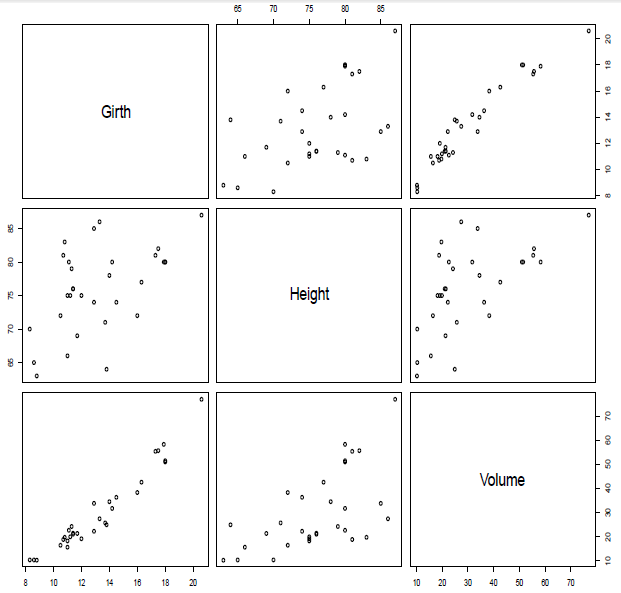
\includegraphics[scale=0.5]{treescatter}
\end{center}


Consider all trees with girth $x_{01}=15\ in$ and height $x_{02}=80 \ ft$ .
\begin{enumerate}
\item Estimate the mean volume among these trees, along with a standard error and $95\%$ confidence interval. $Note: t_{28,0.025}=2.048$
\item Obtain a $95\%$ prediction interval of $y_0$, the volume from an 
individual tree sampled from this population of 80 footers, with girth 15 inches.
\end{enumerate}

\newpage

\begin{large}
\begin{verbatim}
                                    Sum of           Mean
Source                   DF        Squares         Square    F Value    Pr > F
Model                     2     7684.16251     3842.08126     254.97    <.0001
Error                    28      421.92136       15.06862
Corrected Total          30     8106.08387

Root MSE              3.88183    R-Square     0.9480
Dependent Mean       30.17097    Adj R-Sq     0.9442
Coeff Var            12.86612

                        Parameter Estimates

                     Parameter       Standard
Variable     DF       Estimate          Error    t Value    Pr > |t|
Intercept     1      -57.98766        8.63823      -6.71      <.0001
Girth         1        4.70816        0.26426      17.82      <.0001
Height        1        0.33925        0.13015       2.61      0.0145

                    Covariance of Estimates

Variable          Intercept             Girth            Height
Intercept        74.6189461      0.4321713812      -1.050768886
Girth          0.4321713812      0.0698357838      -0.017860301
Height         -1.050768886      -0.017860301      0.0169393298
\end{verbatim}
\end{large}



Recall: Let $\textbf{W}$ denote a $p\times 1$ random vector with mean $\boldsymbol{\mu}_{\textbf{W}}$ 
and covariance matrix $\boldsymbol{\Sigma}_{\textbf{W}}$. Suppose $\textbf{a}$ is a $p\times 1$ (fixed) vector of coefficients. Then 
\begin{center}
\fbox{
\begin{Beqnarray*}
E(\textbf{a}'\textbf{W}) &=& \textbf{a}'\boldsymbol{\mu}_{\textbf{W}} \\
\Var(\textbf{a}'\textbf{W}) &=& \textbf{a}'\boldsymbol{\Sigma}_{\textbf{W}} \textbf{a}.
\end{Beqnarray*}
}
\end{center}

\begin{enumerate}
\item Consider all trees with Girth 15 and Height 80 
To estimate mean volume among these trees, along with an estimated
standard error, take $\textbf{x}_0' = (1, 15, 80)$ and consider
$$\hat\mu(\textbf{x}_0) = \textbf{x}_0'\hat{\boldsymbol{\beta}}$$
$$E(\textbf{x}_0'\hat{\boldsymbol{\beta}}) = \textbf{x}_0' \boldsymbol{\beta}$$
$$Var(\textbf{x}_0'\hat{\boldsymbol{\beta}}) =\textbf{x}_0' \hat{\boldsymbol{\Sigma}} \textbf{x}_0$$
Substitution of $\hat{\boldsymbol{\beta}}$ and $\hat{\boldsymbol{\Sigma}}=MSE(\textbf{X}'\textbf{X})^{-1}$ gives the 
estimates:
\begin{eqnarray*}
\hat\mu(\textbf{x}_0) &=& (1, 15, 80) \left(\begin{array}{c}-58.0 \\ 4.71 \\0.34\end{array}\right) \\
& = & 39.8 \\
\widehat{\Var}(\hat\mu(\textbf{x}_0)) &=& (1, 15, 80)
\left( \begin{array}{ccc}
74.62      & 0.43      & -1.05 \\
0.43      & 0.070      & -0.018 \\
-1.05      & -0.018    &   0.017 \\
\end{array}\right) 
\left(\begin{array}{c}1 \\ 15 \\80 \end{array}\right) \\
& = & 0.72 \\
\widehat{SE}(\hat\mu(\textbf{x}_0)) &=& \sqrt{.72} = 0.849
\end{eqnarray*}
Thus, a 95\% CI is given by 
$$39.8 \pm 2.048*0.849=(38.061,41.539)$$
\item $95\%$ Prediction limits?  Same idea but we add and subtract $t(.025,28)\sqrt{.72 + MS(E)}$.
\end{enumerate}



\end{document}